\documentclass[12pt,a4paper]{ctexart}
\usepackage[final]{pdfpages}
\usepackage{fancyhdr}
\usepackage{lastpage}
\usepackage{xcolor}
\usepackage{cite}
\usepackage{graphicx}
\pagestyle{fancy}
\fancyhf{}
\fancyhead[L]{\textcolor[gray]{0.6}{\leftmark}}
\fancyhead[R]{\textcolor[gray]{0.6}{\rightmark}}
\fancyfoot[C]{\textcolor[gray]{0.6}{第\thepage 页~共\pageref{LastPage}页}}
\renewcommand{\headrulewidth}{0pt}
\renewcommand{\footrulewidth}{0pt}
\setCJKmainfont{SimSun}[AutoFakeBold,AutoFakeSlant]
\setmainfont{TeX Gyre Termes}
\linespread{1.5}
\setcounter{tocdepth}{4}
\setcounter{secnumdepth}{4}
\ctexset {
section = {
name = {第,章},
number = \chinese{section},
},
subsection = {
name = {第,节},
number = \chinese{subsection},
}
}
\date{}


\title{\Huge\textbf{2023年全国大学生信息安全竞赛\\作品报告}}
\begin{document}
\maketitle
\vspace{6cm}
{
    \Large\textbf{作品名称}:\textbf{\underline{\makebox[10cm]{基于TrustZone-M函数级内存地址}}}

    \textbf{\underline{\makebox[13cm]{空间随机化的可信实时系统}}}

    \textbf{电子邮箱}:\underline{\makebox[10cm]{\textbf{213211377@seu.edu.cn}}}

    \textbf{提交时间}:\underline{\makebox[10cm]{\textbf{\today}}}
}
\thispagestyle{empty}
\clearpage
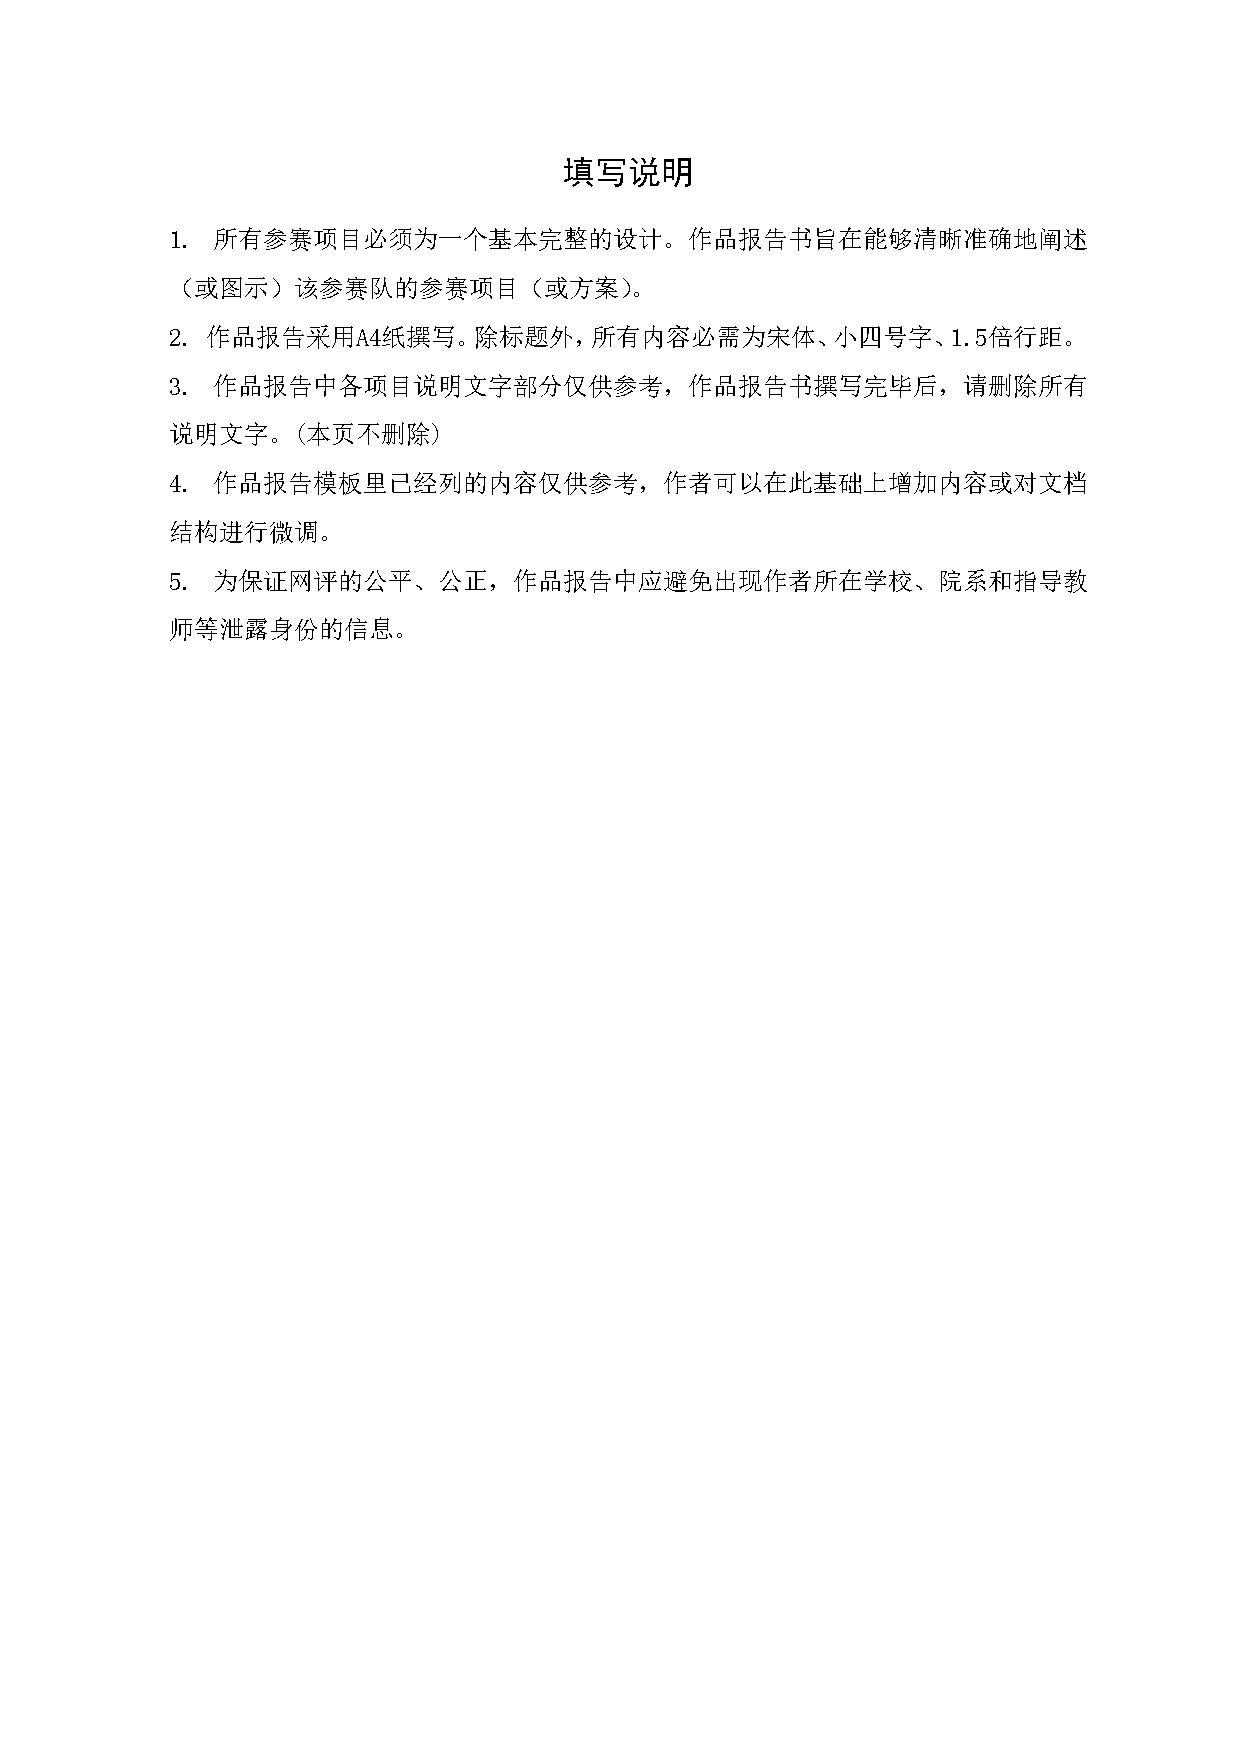
\includepdf{src/request.pdf}
\thispagestyle{empty}
\clearpage
\tableofcontents
\thispagestyle{empty}
\clearpage
\setcounter{page}{1}
\section*{摘要}
\addcontentsline{toc}{section}{摘要}
\thispagestyle{empty}
简要说明创作本作品之动机、功能、特性、创新处、实用性等.
\clearpage
\section{作品概述}
\subsection{作品背景}

\subsection{研究现状}
\par 随着ARMv8-M架构设备在物联网市场的逐渐普及,低端嵌入式系统的安全性近年来受到广泛关注。现有研究主要集中在以下几个关键领域,以解决低端嵌入式系统面临的安全挑战。首先,现有相关研究提出基于TrustZone-M技术的可信执行环境构建技术,其主要目的是为低端嵌入式设备提供可信软件服务,通过安全的通信机制使用户应用程序能够调用安全服务从而提高系统安全性。其次,面向低端嵌入式系统的OTA技术安全风险是一个重要领域,研究人员致力于解决OTA过程中可能面临的各种安全威胁。另外,Trusted firmware-M开源固件项目提供了一个综合性的安全框架,用于保护Arm Cortex-M设备的安全性。此外,面向低端嵌入式系统的内存破坏防御技术针对内存破坏攻击威胁进行研究,主要包括控制流完整性保护和地址空间信息隐藏技术。最后,ASLR(Address Space Layout Randomization)地址空间布局随机化技术提出了一种从另一个角度对系统进行保护的安全技术。这些研究领域的进展对于提高低端嵌入式系统的安全性具有重要意义。
\subsubsection{ASLR(Address Space Layout Randomization)地址空间布局随机化}
\par 自从1988年11月2日莫里斯蠕虫利用缓冲区溢出漏洞感染了上万台计算机之后,安全防护领域涌现出许多针对特定攻击方式的技术,例如StackGuard用于阻止栈溢出,DEP用于阻止代码注入等。然而,这些技术各自只能防御一种特定方式的攻击,要将它们集成在一起实现综合的防护变得困难且具有较高的实施开销。此外,攻击者不断创新,不断出现新的攻击方式,这使得传统的防护技术面临挑战。
\par 为了解决这些不足,研究人员开始探索一种从另一个角度对系统进行保护的安全技术,即地址空间布局随机化(ASLR)。ASLR的核心思想是通过随机化系统的内存布局,使得攻击者无法预测和利用特定的内存地址,从而增加攻击的难度。它引入了一定程度的不确定性和随机性,使得攻击者难以准确定位和利用系统中的关键函数或数据。
\par 具体而言,ASLR通过在系统启动时对代码、堆、栈和库等内存区域的基址进行随机化,使得它们在每次运行时都位于不同的内存位置。这种随机化使得攻击者无法事先获知这些内存区域的准确位置,从而破坏了攻击者依赖特定地址的攻击方式,如代码注入和ROP(Return-Oriented Programming)攻击。
ASLR的实现依赖于操作系统的支持,它需要对内核和应用程序进行修改和扩展。通常,操作系统会提供一种机制来生成随机的内存布局,并在运行时将这些随机值应用于相应的内存区域。此外,ASLR还可以结合其他防护技术,如栈随机化和堆随机化,以提供更强大的保护效果。
\par ASLR最早由Pax项目在2001年作为Linux修补程序创建。其实现方法包括对进程加载时的不同内存区域进行随机化,以使攻击者难以准确定位和利用特定的内存地址。
\par 具体来说,在ASLR的实施中,栈基地址的4-27位共24位会被随机化,而主程序映像、静态数据区和堆这一连续区域的基地址的12-27位共16位以及共享加载库地址的12-27位共16位也会被随机化。通过这种方式,ASLR增加了系统内存布局的不确定性,使得攻击者无法事先获知关键代码和数据的准确位置。
\par 在与数据保护执行(Data Execution Prevention,DEP)结合使用时,ASLR构成了一个完整的系统防护方案。DEP技术迫使攻击者只能使用空间中已有的代码,而ASLR使得这些代码的地址变得不可预测。这样的组合极大地降低了攻击成功的概率,在当时的Linux系统中得到广泛应用。从Windows Vista开始,ASLR也被集成到Windows操作系统中,并随后出现在各种主流通用操作系统中。
\par 然而,在嵌入式系统中,由于其地址空间较小且缺乏像加载器这样的硬件条件,ASLR技术的实施变得相对困难。为解决这个问题,本文提出了以函数为粒度的函数动态随机加载技术,并建立相应的安全执行环境。通过这种方法,嵌入式系统能够在受限的资源和硬件条件下,实现对函数地址的随机化,从而提高系统的安全性。

\subsubsection{基于TrustZonc-M技术的可信执行环境构建技术}
一般来说,可信执行环境由可信执行环境操作系统(Trusted Execution EnvironmentOperating System,TEE OS)以及安全服务(或称为TA,Trusted Application)构成,可信执行环境操作系统主要为用户调用安全服务提供安全的通信机制。ARM TrustZone技术是ARM 公司2008年提出的处理器级系统范围的可信执行环境解决方案,为Cortex-A 系列芯片提供安全的可信执行环境支持。目前,大多数智能手机已配备有TrustZone的芯片以及可信执行环境操作系统,并安装了相应的安全服务以用于手机的安全支付、指纹服务、文件保密等。为了满足低端嵌入式系统对安全日益增长的需求,ARM在2015年提出了面向Cortex-M系列芯片的TrustZone-M8技术并支持ARMv8-M架构设备。基于TrustZone-M的低端嵌入式系统在物联网市场正逐渐普及,然而,面向资源受限设备的可信执行环境研究在学术界和工业界尚处于起步阶段。\\

\subsubsubsection{TrustZone-M 技术的安全机制}
\par TrustZone-M面向资源受限的低端嵌入式设备,利用系统级的硬件隔离技术将系统资源分为安全/非安全世界。安全世界的资源可以访问非安全世界的资源,反之则会产生错误。下面从编程模型、资源分配以及异常处理三方面对TrustZone-M进行介绍。
\par \textbf{编程模型:}自ARMv7-M架构开始,处理器有两种操作模式:thread模式和 handler模式。在thread模式下,处理器用于执行应用程序代码且其访问权限级别可以处于特权态(Privileged)或者非特权态(Unprivileged)。在 handler模式下,处理器用于执行异常处理程序代码且总是特权态。ARMv8-M架构引入TrustZone-M技术后,处理器额外增加了两个安全状态:安全态(Secure State)和非安全态(Non-secure State),这两个状态和处理器操作模式互相独立,即每个安全状态都有thread或者handler两个操作模式。安全状态不是由某一安全位控制,而是取决于处理器所访问的内存地址或者IO地址是映射在安全还是非安全世界。若该内存映射在安全世界,则处理器状态为安全态,反之,则为非安全态。不同的安全状态以及处理器操作模式对应不同的栈指针寄存器,共有 PSP\_NS、PSP\_S、MSP\_NS、MSP\_S 四个栈指针寄存器,程序当前所使用的寄存器由当前处理器的状态决定,其中,thread 模式可以使用PSP (Process Stack Pointer>栈指针寄存器,也可以使用MSP (Main Stack Pointer)栈指针寄存器,而handler模式只能使用MSP栈指针寄存器。此外,支持 TrustZone-M 的ARMv8-M架构为两个安全状态分配了独立的CONTROL寄存器以及异常处理控制寄存器(PRIMASK、FAULTMASK、BASEPRI)。
\par \textbf{安全/非安全世界的切换通过三条新引入的指令实现:}用于从非安全世界跳转至安全世界指令BXNS (Branch and Exchange Non-secure(、安全网关指令SG (SecureGateway)以及用于从安全世界链接跳转至非安全世界指令BLXNS (Branch with Linkand Exchange Non-secure)。安全世界程序调用非安全世界程序一般使用BLXNS 指令,然而,非安全世界程序不能直接调用安全世界程序,它必须首先跳转至该程序在一块特殊的安全世界内存区域的入口,该内存区域被称为非安全可调用(Non-SecureCallable,NSC)区域。为保证入口是从非安全世界至安全世界的有效跳转,入口的第一条指令必须为SG。当安全世界程序执行完成后,使用BXNS指令即可返回至非安全世界。此外,异常处理时也可以发生安全状态的切换。
\par 基于TrustZone-M设备的系统运行机制如下图所示,当设备上电启动之后,首先会执行安全世界的固件程序,包括安全启动(①)以及TrustZone-M的初始化,其中,TrustZone-M 的初始化主要涉及对资源的安全属性划分与配置。然后,由安全世界将控制权转交给非安全世界的启动代码并进行非安全世界的初始化。在此之后,系统运行非安全世界的应用程序,在运行过程中,非安全世界可以通过调用安全世界的API以在安全世界执行相应任务,同样的,安全世界在执行过程中也可以通过回调函数调用非安全世界的函数。
\begin{figure}[h]
    \centering
    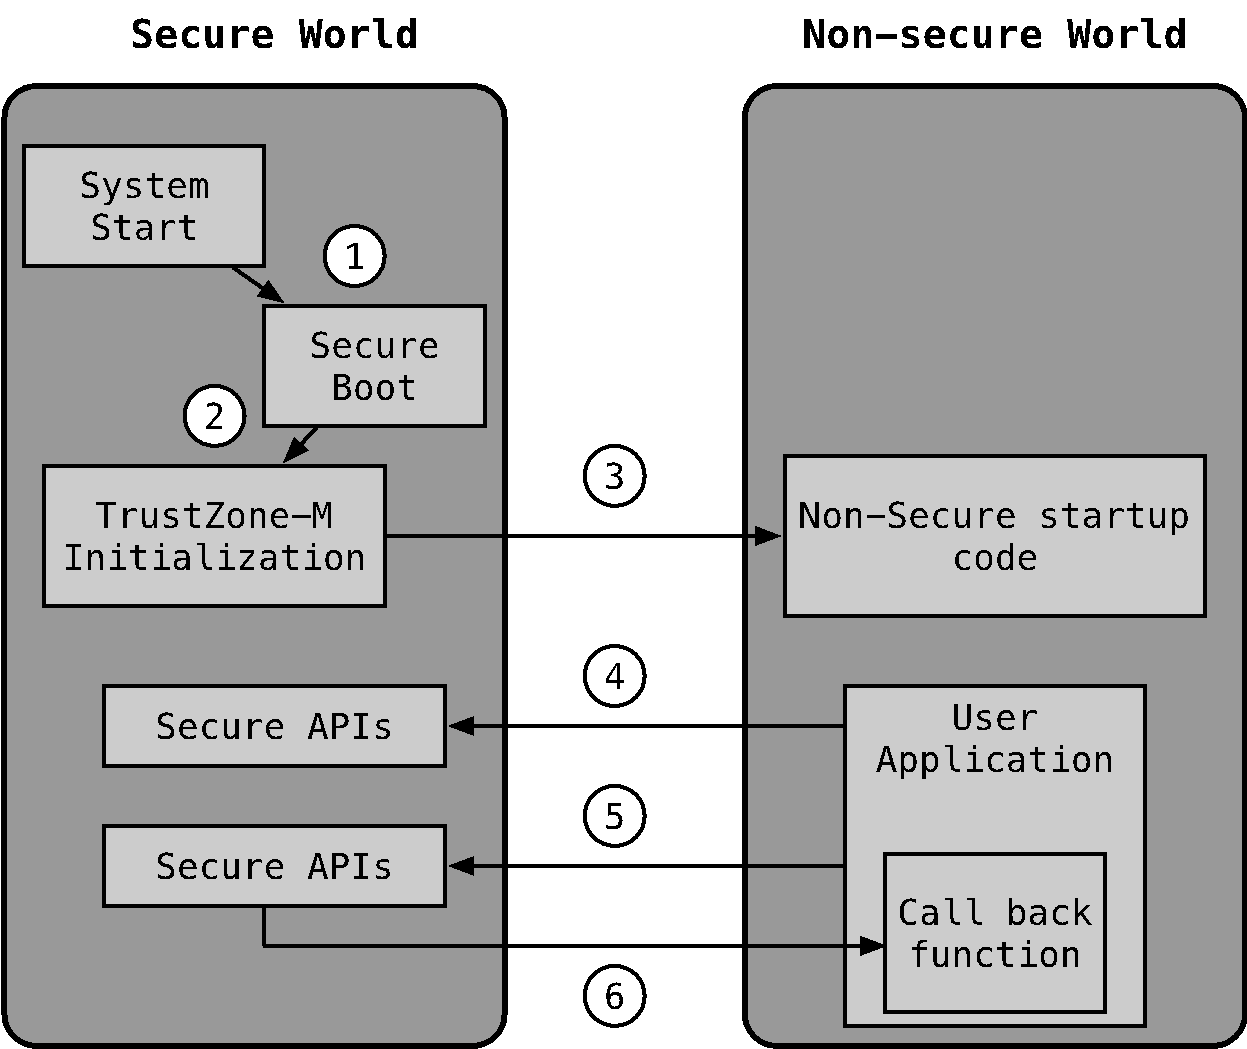
\includegraphics[scale=0.5]{graph/2.png}
    \caption{基于TrustZone-M的系统运行机制}
\end{figure}
\par \textbf{资源分配:}TrustZone-M 技术为ARMv8-M架构设备提供基于硬件的内存隔离机制,处理器根据内存映射可以对所有资源(包括内存,外设等)进行访问,其内存资源可以设置不同的安全属性以及资源访问控制权限。内存资源可以通过安全属性单元(Security Attribution Unit,SAU)进行安全区域的划分,区域数量由芯片制造商决定,一般为8个区域,SAU只能在处理器处于安全状态下被配置。除SAU之外,安全属性还可以通过实现定义属性单元(Implementation Defined Attribution Unit,IDAU)来进行配置。对某一内存区域来说,其安全属性取决于SAU和IDAU对其配置的共同作用结果,通过对两种配置取逻辑或操作以确定最终的安全属性。此外,内存资源可以通过内存保护单元(Memory Protection Unit,MPU)进行内存访问权限的设置,包括读权限、写权限、可执行权限。任何未遵守该权限要求的访问将会触发HardFault 异常处理,安全/非安全世界各有一个MPU。
\par \textbf{异常处理:}在支持‘TrustZone-M 的设备上,通过嵌套向量控制器(Nested VectorInterrupt Control,NVIC)可以设置异常处理为安全或者非安全属性。ARM的M系列处理器在异常处理时支持硬件级的异常上下文保存与恢复。TrustZone-M 的异常处理操作模式切换如图1-2所示,一旦异常被触发,处理器根据向量表(Vector Table)决定异常处理程序并进行控制流跳转,其操作模式自动切换成handler模式并且使用MSP作为异常处理时的栈指针,而异常触发前的上下文信息会自动的压入在先前执行的栈中,称为异常栈帧(Exception Frame)。在ARMv8-M Baseline 架构下的异常栈帧的结构如图1-3所示,包括状态寄存器xPSR、异常返回地址、链接寄存器LR以及通用寄存器RO-R3的值。同时,当前链接寄存器LR将会载入一个称为EXE\_RETURN的特殊值,该特殊值记录着异常返回时处理器的状态信息,如处理器的操作模式、安全状态、使用的栈寄存器等。当异常返回(即跳转至EXE\_RETURN)时,异常栈帧中的内容会自动的载入其对应的寄存器中以恢复异常触发前的上下文,控制流也回到异常触发前的位置继续执行。\\

\subsubsubsection{基于TrustZone-M的可信执行环境研究应用}
\par 迄今为止,已有相关公司以及研究团队利用TrustZone-M技术提出面向资源受限设备的可信执行环境。Trusted Firmware-M (TF-M)是ARM公司针对ARMv8-M架构包括Cortex-M23,Cortex-M33,Cortex-M55处理器)或者双核平台提供的一个基于双世界架构(即安全世界和非安全世界)的可信执行环境。它符合ARM公司为物联网嵌入式系统提出的首个行业安全平台架构 PSA Platform Security Architecture)标准,并由ARM公司主导开源。TF-M在ARMv8-M架构上利用TrustZone-M 的隔离机制将程序执行环境划分为非安全处理环境(Non-secure Processing Environment,NSPE)以及安全处理环境(Secure Processing Environment,SPE)。在安全处理环境中,TF-M为用户层提供多种安全服务,比如安全启动、安全密钥、安全存储等。其内核层利用SAU以及MPU对安全服务之间进行运行时隔离,并为安全服务之间以及NSPE与安全服务之间提供了安全的通信、安全中断处理等机制,NSPE中的程序可以通过TF-M提供的PSA功能API对安全服务进行调用。然而,用户程序对安全服务进行调用时会进入阻塞直到调用结果返回,这是因为TF-M为满足PSA提出的高等级隔离,TF-M中安全服务的调用模型为信号驱动型且由TF-M 内核提供进程间通信( Inter-processingCommunication,IPC)机制负责与安全服务进行交互。
\begin{figure}
<<<<<<< HEAD
    \centering
    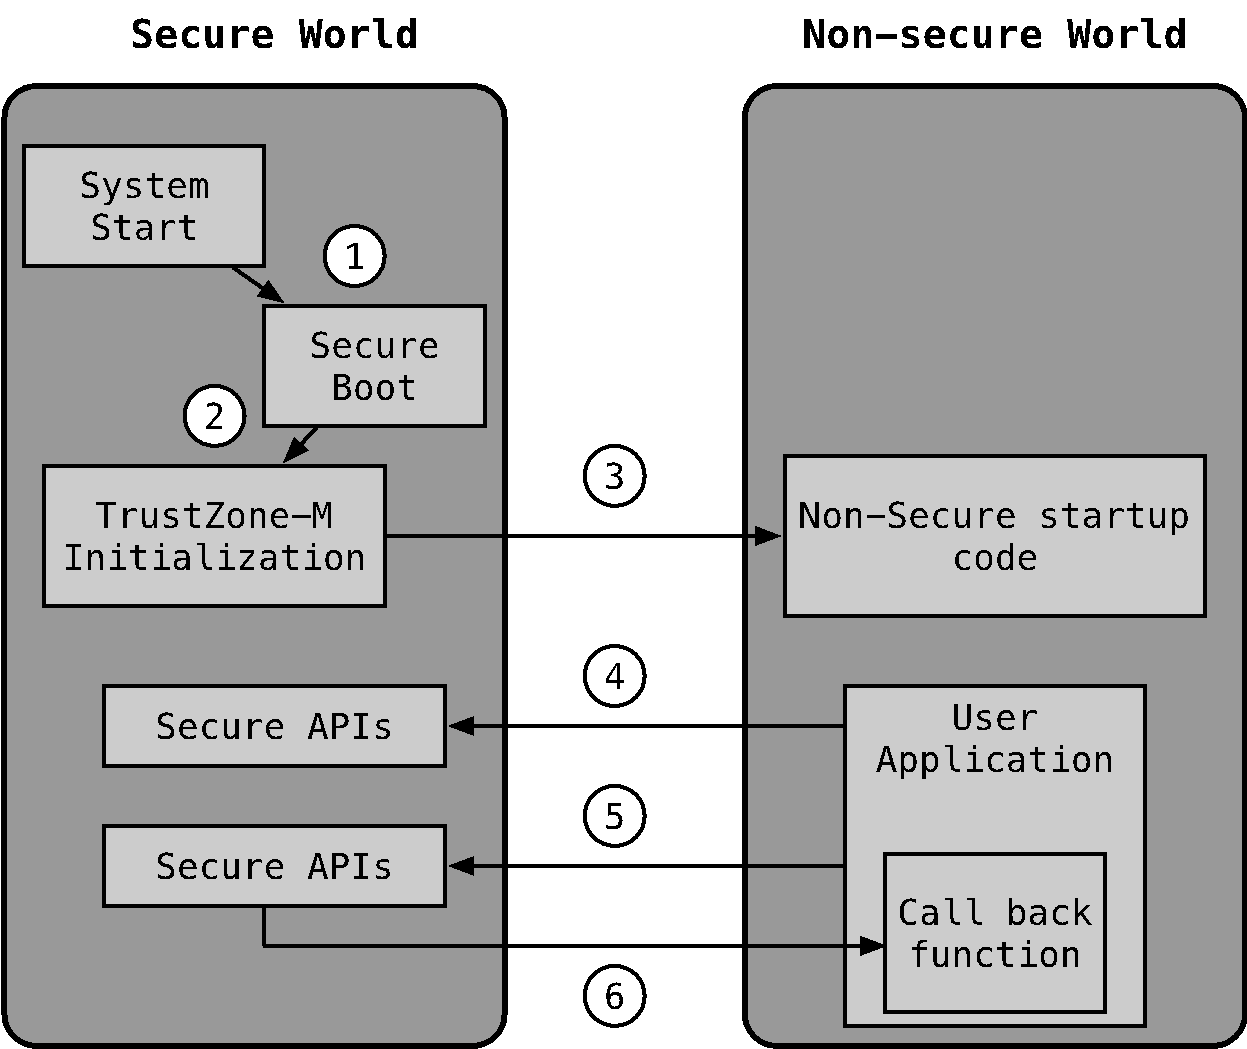
\includegraphics[scale=0.5]{graph/2.png}
    \caption{基于TrustZone-M的系统运行机制}
=======

>>>>>>> 2bc8b46690a640fb173aa1dab7968bee48763b1b
\end{figure}
\par Trustonic公司与Microchip公司联手推出了基于TrustZone-M的 Knibi-M双世界架构可信执行环境,它针对裸机版本的SAML1120l设计开发,用于为该设备提供可信的安全服务。它包括内建的密码算法和安全数据存储,可以被集成到支持TrustZone-M的不同微处理器上。Knibi-M利用TrustZone-M以及安全网关(Secure Gateway)[21以与传统的非安全世界应用进行隔离。安全世界包括Knibi-M引导(Bootloader)以及多个安全服务的操作系统,可以为非安全世界中的应用程序提供安全的功能。非安全世界包括主要的应用程序以及调用安全服务的接口。Knibi-M含有一个设备唯一的密钥(目前仅支持SAML11 KPH版本),它是设备出厂时由制造商安装的,它可以为Knibi-M提供消息证明,证明的消息可以被‘Trustonic 的云服务商认证,从而证明该消息来自一个已知的设备。目前,Knibi-M只支持裸机版本 SAML11,并不支持其他型号的ARMv8-M 设备且未支持实时操作系统。

\par Oliveiral22l等人利用‘TrustZone-M 技术,针对ARMv8-M 设备提出了基于多世界(Multi-world)架构的可信执行环境操作系统UTANGO。它根据最小权限原则,利用TrustZone-M的安全状态控制器(即SAU或 IDAU)降低安全服务的执行权限并使其在非安全世界下执行,并为非安全世界的程序以及各个安全服务提供互相隔离且相同的运行环境,该运行环境称为非安全虚拟世界(Non-secure Virtual World,NSVW)。为了能切换不同的 NSVW,每个NSVW都有一个世界控制块(World Control Block,WCB)用于记录其上下文内容,系统运行时UTANGO在安全世界为非安全世界运行的所有NSVW进行调度并为各个NSVW之间提供数据通信接口。然而,由于在世界切换过程中涉及大量的上下文内容保存与恢复,为系统带来较严重的性能开销。另外,目前UTANGO暂不支持抢占式世界切换,非当前NSVW产生的异常难以得到及时的处理,对系统实时性有一定影响。
\par 现有TrustZone-M的可信执行环境的相关工作,其功能主要是为安全服务提供可信的执行环境并为用户提供基于不同安全通信机制的安全服务调用。然而,目前开源可信执行环境中的安全通信机制交互过程复杂,相对于资源和性能受限的低端嵌入式系统来说具有较大代码和性能开销,且可扩展性较差,例如TF-M的信号驱动型安全服务以及IPC的通信机制、UTANGO中NSVW之间繁重的上下文切换等。除此之外,现有基于双世界架构的安全通信机制只允许执行单个安全服务,并未考虑实时操作系统环境下多任务对安全服务进行并发调用需求,导致多任务下对安全服务的调用易受到阻塞,对多任务间的实时协同性产生影响。然而,TF-M 以及Knibi-M 的安全通信中对安全服务请求过程的参数检查,隔离机制等为本论文设计安全通信机制提供了一种可行思路。另外,本论文针对现有可信操作系统未支持多任务场景下安全服务的并发调用问题,基于现有实时操作系统FreeRTOS,设计多任务场景下对安全服务的并发调用技术。


\begin{figure}[htbp]
    \centering
    \begin{minipage}[t]{0.4\textwidth} %textwidth值小于0.25,或者linewidth小于0.5,不过这里设置textwidth比设置linewidth效果好一些
        \centering
        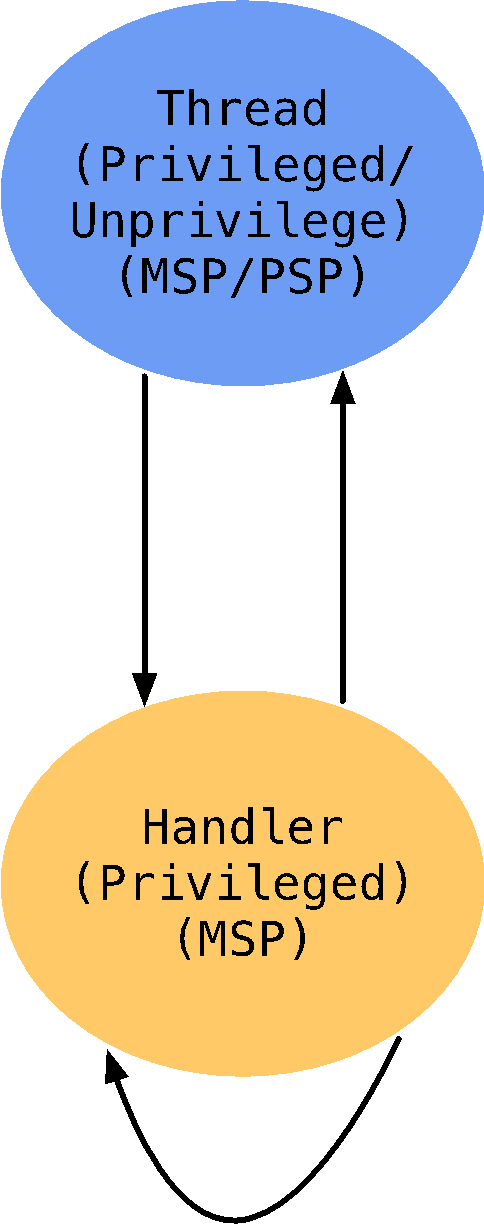
\includegraphics[scale=0.25]{graph/3.png}
        \caption{异常处理操作模式切换}
    \end{minipage}
    \hspace{0.58in} % 两图片之间的距离
    \begin{minipage}[t]{0.4\textwidth}%textwidth值小于0.25
        \centering
        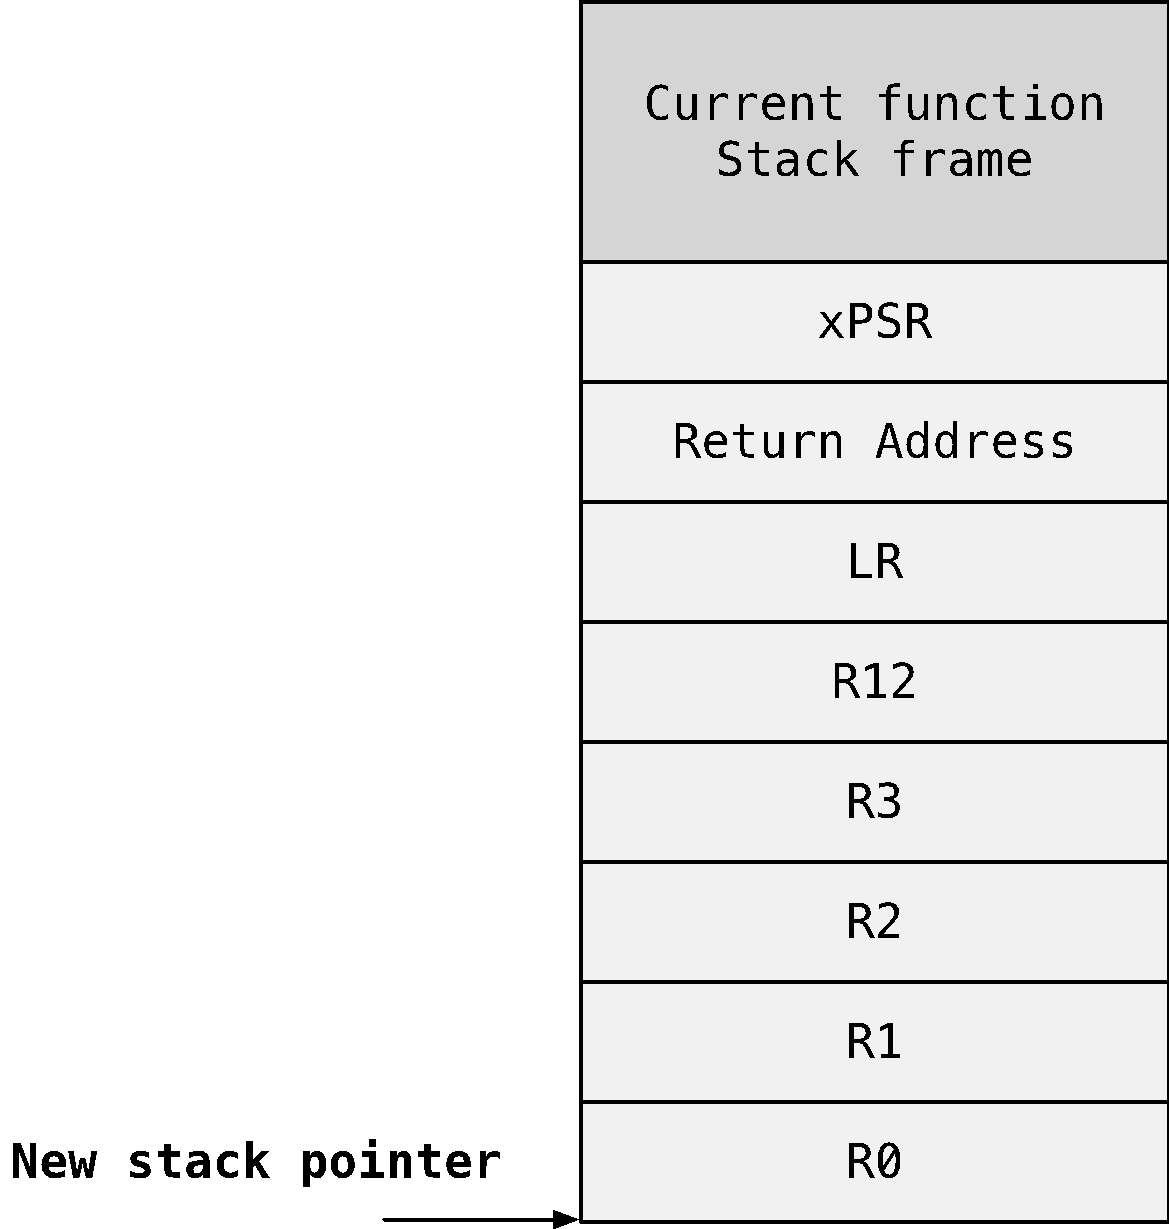
\includegraphics[scale=0.25]{graph/4.png}
        \caption{异常帧栈结构}
    \end{minipage}
=======
\begin{figure}

>>>>>>> 2bc8b46690a640fb173aa1dab7968bee48763b1b
\end{figure}

\par 在Trusted Firmware-M的背景下,安全启动负责在固件映像被加载和执行之前验证其真实性和完整性。它通过根据设备安全引导固件中存储的一组受信任的密钥检查固件映像的数字签名来执行此验证。安全启动可以对SPE (Secure Processing Environment)和 NSPE (Non-Secure Processing Environment)固件映像进行身份验证。NSPE映像在设备的非安全世界中执行,而SPE映像在安全世界中执行。如果固件映像未通过Secure Boot验证,则会被拒绝,设备将无法执行它。这可以防止攻击者在设备上执行未经授权的代码,从而保护设备及其数据免受恶意活动的侵害。
\par TF-M内核是TF-M的主要组成部分之一,它是一个基于微内核的安全操作系统内核。TF-M core的主要功能是提供安全隔离、通信控制和安全执行,主要模块包括IPC、SPM、Interrupt Handling。其中,IPC 用于在SPE和 NSPE之间进行通信。它提供了一种安全的方式,以便在受保护的环境内传递数据和控制信息。SPM用于管理和控制在SPE中运行的各个安全分区。SPM使得多个安全分区可以在同一硬件平台上运行,并且可以互相隔离。Interrupt Handling用于管理和处理来自设备的中断请求。TF-M内核通过在SPE和NSPE之间传递中断请求,确保了所有中断的安全处理。TF-M内核还包括一些其他的辅助模块,比如Secure Entry/Exit和Secure Attribution等,用于在SPE和NSPE之间进行安全的上下文切换和资源分配。
\par 安全服务负责向安全/非安全世界提供具有较高安全需求的功能实现并由安全内核负责对其进行调用,如安全储存、安全启动、加密等。每一个安全服务具有唯一标识符SID(Service ID)且有统一的函数调用入口。为统一调用接口,每个安全服务都可以通过SID和version两个参数被非安全世界用户进行调用,其中,SID参数是要调用的安全服务的唯一标识符,version是请求的信任根服务版本。NSPE的用户通过PSA API发送请求后,由SPM将请求打包成消息并转发到相应服务处理程序的函数。
\par 非安全世界在调用安全世界的安全服务时,其整个通信过程如下图所示,可以分为三个阶段:(1)请求阶段:非安全世界任务发起安全服务的请求至特定的API并最终交给TF-M内核;(2)执行阶段:TF-M内核验证客户端的身份和权限,然后根据请求中指定的安全服务标识符,将请求转发给对应的安全服务并等待其响应结果;(3)响应阶段:安全服务执行结束并返回执行结果给 TF-M内核,TF-M内核收到安全服务的执行结果后,会根据请求的类型和参数,将结果通过特定API返回给客户端。\\
\subsubsubsection{TF-M应用研究}
\par 2016年,P. Wägemann等人(A TrustZone-Based Secure Firmware for IoT Devices" - P. Wägemann, M. Cremers, and S. Mangard (2016))设计和实现一种基于TrustZone的安全固件架构,利用TF-M作为基础来保护物联网设备免受各种攻击。该安全固件架构基于TrustZone技术,该技术提供了硬件级别的安全隔离。研究者利用TrustZone的两个不同的执行环境,即"安全世界"和"非安全世界",来实现安全隔离。安全世界运行在受保护的安全模式下,而非安全世界则运行在常规的非安全模式下。通过使用TrustZone和TF-M,研究者实现了更强大的安全隔离。安全世界被限制为只能通过安全接口与非安全世界进行通信,这确保了安全世界的代码和数据无法被非安全世界访问或篡改。安全世界中的关键功能和数据被保护在一个安全的容器中,只有经过授权的访问才能获取。为了保护设备中的关键数据和执行,研究者采取了多种安全措施。首先,通过在安全世界中运行关键功能,确保只有经过授权的代码可以访问和执行这些功能。其次,使用加密算法对关键数据进行加密,以防止未经授权的访问。此外,安全世界中的代码和数据也可以受到完整性检查的保护,以确保其未被篡改。但这项研究可能存在一些实施上的挑战。例如,由于物联网设备的资源限制,安全固件的实现可能会受到性能和存储限制的影响。此外,研究中可能没有对所有可能的攻击进行全面考虑,导致可能存在其他安全漏洞。
\par S.Kumar等人进行的研究(Enabling Secure Firmware Updates for IoT Devices using ARM TrustZone" - S. Kumar, S. Mukhopadhyay, and M. Saxena (2019))旨在解决物联网设备固件更新过程中的安全性问题。研究者提出了一种安全的固件更新机制,利用ARM TrustZone和TF-M来确保固件的完整性和机密性。他们采用了多种机制来防止恶意固件的注入。首先,实现了固件验证机制,通过数字签名或哈希算法对固件进行验证,确保固件的完整性。只有通过验证的固件才能被接受和安全地更新。其次,实现身份认证机制用于验证固件的来源和合法性,以防止非法固件的注入。这可以通过使用公钥基础设施(Public Key Infrastructure)或其他身份验证机制来实现,确保请求只有来自信任的源头才能被接受。通过使用ARM TrustZone和TF-M,研究者确保了固件更新过程的安全性。安全世界中的代码负责处理固件更新的操作,并通过安全接口与非安全世界进行通信。固件在安全世界进行验证和认证后,才能被接受并安全地更新到设备中。这样可以防止未经授权的固件更新,同时确保更新的固件是合法和可信的。但本研究实现的安全固件更新机制在实现过程中无法确保在固件更新过程中,包括固件的验证、加载和替换过程的所有环节都是安全的。
\par  Arm Limited 公司("Trusted Firmware-M: A Comprehensive Security Framework for Arm Cortex-M Devices")基于前人的研究,为物联网设备提供一个全面的安全框架,提供了全面的安全功能应用,以应对不断增长的安全威胁。Arm Limited 的研究方案主要集中在设计和实现 TF-M 的安全特性和功能。这些功能包括安全引导(Secure Boot)、安全分区(Secure Partitioning)和安全通信(Secure Communication)等。相较于以往的研究,Arm Limited 在 TF-M 的研究中取得了一些突破。他们提供的全面安全框架集成了安全引导、安全分区和安全通信等关键功能,使得物联网设备能够综合地应对安全挑战。其次,他们基于 Arm Cortex-M 架构,充分利用硬件安全特性和 TrustZone 技术,提供了更强大的安全隔离和保护机制。但是,尽管 Arm Limited 的研究提供了一个全面的安全框架,但也存在一些限制和挑战。例如,由于物联网设备的多样性和复杂性,将该安全框架应用于不同设备可能需要定制化的适配和配置,这将增加了开发和部署的复杂性。此外,该研究可能没有充分考虑到未来可能出现的新型安全威胁和攻击方式。
\par J. Kim等人的研究("Secure Bootloader Design for IoT Devices using Trusted Firmware-M")旨在设计一种基于 TF-M 的安全引导程序,以提供物联网设备的安全引导功能。研究者设计了一个基于 TF-M 的引导程序,该程序能够确保设备在启动过程中的安全性,并保护设备免受恶意固件的加载和执行。研究者利用 TF-M 提供的安全特性,如安全分区和安全存储,来实现安全引导过程。安全隔离使引导程序运行在安全分区中,与非安全分区进行隔离。这样可以防止恶意固件或非授权代码对系统的攻击和篡改。只有通过授权的引导程序可以加载和执行,确保引导过程的完整性和可信性。安全验证使引导程序和关键数据存储在安全存储中,并通过安全存储的保护机制进行访问控制。在引导过程中,TF-M可以验证引导程序的完整性和真实性,确保只有经过验证的固件被加载和执行。然而,这项研究还存在一些潜在的缺陷和不足,比如如何确保引导程序的完整性和可信性,以及应对物理攻击和侧信道攻击的挑战。此外,实施安全引导可能需要额外的硬件支持或安全认证机制,将增加设备的成本和复杂性。

\subsubsection{面向低端嵌入式系统的内存破坏防御技术}
\par 内存破坏问题一直是计算机安全领域研究的重点之一,它一般存在于C或者C++编写的软件中,内存破坏攻击都是通过触发一个内存错误以实现攻击,比如悬挂指针,数组越界访问等。根据Szekeresl28等人对内存破坏攻击的调研,攻击者可以利用内存破坏漏洞实现代码破坏攻击(Code Corruption Attack),控制流劫持攻击(Control-flowHijack Attack),面向数据的攻击(Data-only Attack)以及信息泄露攻击( InformationLeak Attack)。其中,尽管在低端嵌入式系统安全领域已存在些许安全机制以抵御不同类型的内存破坏攻击,然而,控制流劫持攻击依旧是该领域的主要威胁,现有针对控制流劫持攻击的防御中,主要以控制流完整性保护技术以及地址空间信息隐藏技术最具代表性。\\
\subsubsubsection{控制流完整性保护技术}
\par 控制流完整性保护技术是指对控制流转移进行检查以防御控制流劫持攻击。控制流劫持攻击是由于内存安全问题所引起的针对间接控制流转移的篡改,目前可分为前向控制流转移攻击和后向控制流转移攻击。前向是指攻击者通过篡改函数指针或者虚函数表等来达到转移控制流的目的,而后向则是指通过篡改函数返回地址来改变控制流转移,因此控制流完整性保护可分为前向控制流完整性保护以及后向控制流完整性保护。由于前向控制流完整性保护性能很大一部分取决于CFI的目标集(即CFI所保护的间接跳转的集合)中产生调用的次数,而对于低端嵌入式系统来说,其代码量较少,导致其CFI目标集也相对较少,因此可以通过直接部署通用系统的前向完整性保护技术l80以保证前向控制流完整性。然而,对于基于返回地址的后向完整性保护来说,函数的返回地址由于其在程序中所占数量庞大,且更容易被攻击者所利用,因此后向完整性保护在低端嵌入式系统领域依然具有较大的挑战性。
\par Sun 等人I31l针对嵌入式系统提出了操作完整性(Operation Execution Integrity ,OEI),并设计了一个端到端的系统OAT (OEI ATtester),该系统可在基于ARM 的嵌入式设备上实现OEI的远程认证。OEI包括控制流完整性以及数据流完整性。在控制流完整性上,OAT利用远程证明机制来提高在嵌入式设备上的性能,它结合对控制流转移以及返回的跟踪,计算其相对应的哈希值并发送给远程验证服务器,保证对控制流完整性前向和后向的双覆盖,使远程验证者能够快速地重构控制流并对其完整性进行验证。然而,该防御机制需要额外硬件支持(比如可信执行环境,额外的处理器核心等)并且仅能够检测攻击但不能终止攻击。在针对后向控制流完整性保护的研究中,影子栈被证明可以提供对返回地址的完整性保护,因此受到广泛关注。CFI-CaRE利用TrustZone-M技术将影子栈进行强制硬件隔离从而实现后向完整性保护,每次对影子栈的操作需要面临一次系统调用以及一次安全/非安全世界的切换。RECFISHI结合CFI技术以及影子栈并通过插桩技术直接应用到嵌入式系统的二进制文件上,从而不需要源码的支持,但是由于它将影子栈部署在特权区域( Privileged Region),所以每次函数返回时必须经过一次系统调用。因此,这两种方法都面临较大的性能开销。随后,Silhouettel3S利用平行影子栈(Parallel Shadow stack)36技术镜像一个相同大小的栈,使用MPU对影子栈以及用户代码区域进行权限划分,最后利用基于ARMv7-M指令集的存储硬化(Store Hardening)技术对用户代码区域进行权限转换,从而保证影子栈与用户代码的地址空间隔离。但受限于ARMv7-M指令集,部分指令的转换(例如浮点存储指令)会带来较大的空间和时间开销。除了利用影子栈实现控制流完整性保护,Werner等人l37提出了一种基于海绵的控制流保护(Sponge-based Control Flow Protection,SCFP)。SCFP利用RISC架构的硬件扩展在CPU取指和译码阶段插入控制流完整性检查。SCFP通过对指令的加密和解密来认证控制流的完整性,但由于它仅仅防御控制流后向攻击而不能像影子栈一样保证返回地址完整性,因此控制流弯曲攻击(Control-flow Bending Attack)139对其依旧有效。随后,uRAI[2通过保留一个专用寄存器来存放返回地址以保证返回地址的完整性。由于其不需要一个受保护的影子栈或者可信执行环境,因此 uRAI在大多数的函数调用过程中有较高的效率且适用于大多数嵌入式系统,但是对于异常处理函数施加软件错误隔离(Software-Fault Isolation,SFI)B38]以及函数嵌套调用使得单一寄存器进行分段处理,导致复杂性大大增加,从而对性能具有较大影响。
\par 目前该类防御技术侧重于保证后向控制流的完整性,这些技术利用分配一块区域(如影子栈、专用寄存器等)用于存储返回地址并利用隔离机制以保证该区域的安全性。一般来说,这些技术需要对代码进行转换或者相应硬件支持以将返回地址存储于上述安全区域,依赖于设备处理器架构,难以直接扩展至ARMv8-M架构。\\
\subsubsubsection{地址空间信息隐藏技术}
\par 由于控制流劫持攻击的一般前提是攻击者已知被攻击设备的固件程序地址空间信息并借助该信息以实施攻击,比如ROP攻击通过利用代码段地址空间信息构成ROP链以达到最终攻击目的,因此,地址空间信息隐藏技术通过保护在设备内存中运行的程序地址空间信息,如代码段内容及位置等以防御控制流劫持攻击。目前在低端嵌入式系统领域的相关安全研究中,地址空间信息隐藏技术主要有两种方式:内存只可执行XOM (Execute Only Memory)I40以及软件多样化(Software Diversification)。
\par XOM旨在使程序的代码段只可执行而不能被读写,从而防止代码段地址空间信息的泄漏。不同于通用系统有相应硬件可以对特定内存区域设置XOM属性,低端嵌入式系统受限于其硬件资源,无法实现XOM属性。MPU虽然能实现对内存进行权限上的划分,但是读取权限与执行权限不能够分开,因此单独使用MPU无法实现XOM机制。PCROPR提出了一个面向Flash内存可编程特性的方法,可以保护Flash内存不被用户代码读取但依旧可以被执行。但是,PCROP只对STM系列微处理器有效,具有较小的可扩展性。另外,它只支持Flash 内存而不支持其它类型的内存(如RAM内存)。Braden等人提出了LR2,其基本思想是基于SFI来实现XOM属性并对代码指针进行随机化来防止代码段的信息泄漏。kR\^X基于与SFI相似的代码检查来实现对内核代码的多样化以及XOM属性。这两种方法本质上都是属于基于软件实现的XOM,因此不可避免的会带来严重的性能开销。后来,这两种基于SFI机制的XOM实现还被Kwon 等人lA5证明可以被绕过。同时,Kwon等人提出面向低端嵌入式系统的uXOM,在ARM Cortex-M 系列处理器上实现XOM。通过将加载指令转换为特殊的无特权加载指令I0并利用MPU将代码区域设置为无特权加载指令不可读,从而保证代码段只可执行,但不能被读取。为了保护MPU配置段寄存器不被修改,uXOM使用与之前同样的方式将存储指令也做相应转换。但由于一部分加载/存储指令没有相对应的无特权加载/存储指令,因此需要编译器做额外的代码插桩,带来一些额外的开销。经过测试,uXOM在性能上优于基于SFI的XOM实现。随后,Shen等人提出 PicoXOM,一种利用Cortex-M处理器的调试单元在低端嵌入式系统上实现XOM 的方案,与uXOM一样,兼容所有ARMv7-M 以及ARMv8-M架构的设备。首先,PicoXOM使用MPU将代码段配置成不可写,然后,利用ARM 调试单元中的数据观察点和跟踪( DataWatchpoint and Tracing,DWT)单元,对读取所保护的代码段操作触发异常从而对具体操作进行合法性检查,实现对代码段的读取保护但不影响其执行。由于利用DWT这一硬件特性进行异常捕获,代码正常运行时性能几乎不受影响,并且不需要额外的代码插桩,因此PicoXOM相比uXOM具有较小的性能开销以及额外的代码开销。但由于DWT单元中比较器数量的限制,在保护MPU 配置区域的安全性的前提下,PicoXOM只能应用于代码大小不超过64KB的设备上。
\par 软件多样化是利用编译器优化手段或者运行时随机化技术,在不改变软件功能的前提下,使得该软件的地址空间布局在不同系统上或者在每次执行时呈现多样化,以增加攻击者对软件漏洞的利用难度。现有面向低端嵌入式领域的软件多样化技术主要侧重于启动阶段和编译阶段的多样化。启动阶段多样化技术的典型代表是 AVRAND和MAVRI,它们针对Atmel AVR架构嵌入式设备,在启动阶段引入代码多样化技术以达到对Flash内存布局的随机化。其实现方法是通过静态分析预先获得控制流转移相关的指令以及数据(如函数指针、虚函数表等)并在随机化后对该指令与数据进行重定位。但由于这两种方法都是基于对Flash内存的重写,因此大大降低了嵌入式系统的使用寿命。EPOXYP9)是一种编译阶段的代码多样化技术,该技术针对ARM 架构的低端嵌入式系统,它利用LLVM编译器对函数的位置,数据段以及寄存器的使用进行随机化,并通过安全栈(SafeStack)保护返回地址以抵御缓冲区溢出攻击。相似的工作还有uArmor,其面向低端嵌入式系统并对实时操作系统进行支持,除了对函数、寄存器进行编译阶段的乱序之外,它还实现栈警惕标志(Stack Canary)机制以抵御缓冲区溢出攻击。EPOXY和uArmor通过在编译阶段为不同的设备提供不同的固件以抵御大规模攻击。
\par 此类技术通过保护程序地址空间信息的方式来增加攻击者发现与利用漏洞的难度,以达到抵御控制流劫持攻击的目的。现有软件多样化技术主要侧重于在系统启动阶段以及编译阶段引入多样化技术。然而,由于启动阶段的软件多样化技术需要在启动阶段对主程序执行多样化,而该启动代码本身并未进行多样化,其安全性难以得到保证,攻击者可以利用这一点破坏整个系统的安全性;编译阶段的多样化尽管可以有效防止大规模的攻击,但受限于低端嵌入式系统较小的内存空间难以提高其随机嫡。另外,OTA技术的普及导致更新阶段成为固件信息泄漏的一个关键途径,XOM技术由于其主要目标是在运行阶段防御固件读取攻击以防御控制流劫持攻击,而编译阶段的软件多样化发生在OTA更新过程之前,因此这两种方法都无法防御离线阶段的固件读取攻击。然而,软件多样化技术通过对固件的内存布局进行随机化以隐藏其地址空间信息,最终抵御控制流劫持攻击,为本论文针对低端嵌入式系统固件进行运行时随机化提供了一种可行思路。此外,结合OTA所导致的固件读取攻击,为本论文针对OTA更新过程进行固件随机化提供了现实意义。
\subsubsection{研究现状总结}
\par 现有研究工作在面向内存破坏攻击的通用系统防御技术,基于TrustZone-M技术的可信执行环境构建技术以及面向低端嵌入式系统的内存破坏防御技术方面都已取得一定的进展和成果,发现不同的技术均有其优缺点,对本论文研究工作的开展有很大的借鉴价值,现状总结如下:
\begin{itemize}
    \item[(1)] 当前针对TrustZone-M技术的TEE OS研究尚处于起步阶段,其安全通信机制在设计上存在安全冗余,对低端嵌入式系统具有较大性能开销。此外,现有技术针对安全服务调用暂不支持多任务并发,影响系统多任务实时协同。
    \item[(2)] 现有OTA技术在更新过程中端到端的安全性难以保证,固件在更新过程中可能被攻击者所获取并对其进行逆向分析从而挖掘其中存在的安全漏洞,最终在固件所在设备上实现漏洞利用。
    \item[(3)] 现有地址空间信息隐藏技术均存在安全隐患。由于基于启动阶段的软件多样化技术并未对多样化部署代码进行多样化且缺乏可信根(Root of Trust) ,因此无法保证其自身的可信,攻击者可能利用该代码执行代码复用攻击以破坏系统安全性;基于编译阶段的多样化技术由于资源限制具有较小随机嫡,且其易受到暴力破解攻击。XOM技术通过运行时无法对固件进行读取从而防御地址空间信息泄漏,然而其与编译阶段的多样化技术一样,无法防御离线固件读取攻击,比如OTA更新时的固件泄漏攻击。
\end{itemize}
\subsection{作品意义与目标}

\subsection{应用前景分析}

\section{作品设计与实现}

\subsection{系统架构设计}

\subsection{系统实现方案}
\subsubsection{Trusted firmware-M系统架构}
\subsubsubsection{TF-M简介及设计目的}
\paragraph{(1)TF-M简介}\mbox{}\\
\par Trusted Firmware-M(TF-M)是由Arm开发的开源固件项目,旨在为物联网(loT)设备提供安全的运行环境。TF-M旨在提供一个可配置和可裁剪的安全固件平台,以支持从小型嵌入式设备到高端安全系统的多种应用场景。TF-M的架构是模块化的,允许使用者在不影响其他模块的情况下添加或删除安全服务。
\par TF-M 采用了两个核心概念:Secure Processing Environment(SPE)和Non-Secure Processing Environment(NSPE)。SPE 是一个安全执行环境,可以保护关键数据和代码免受未经授权的访问和修改。NSPE 是一个普通的执行环境,可以访问所有的硬件资源。TF-M 提供了一组安全服务,例如安全启动、加密解密、密钥管理、认证和授权等,这些服务可以在SPE中运行,以保证安全性。

\paragraph{(2)TF-M设计目标}
\par TF-M的设计目标是保护互联网设备上的敏感数据和代码免受攻击,它需要满足以下需求:
\begin{itemize}
    \item 安全性:TF-M 旨在为 IoT 设备提供安全的运行环境,以保护设备和用户数据免受攻击。
    \item 可配置性:TF-M 的架构是模块化的,允许用户根据自己的需求配置和定制安全服务。
    \item 易于集成:TF-M 提供了一个标准接口,使得其他软件可以轻松地与TF-M 集成。
    \item 可移植性:TF-M 可以在不同的硬件平台上运行,并且支持多种处理器体系结构。
    \item 易于维护:TF-M 的代码是模块化的,易于理解和维护。
\end{itemize}

\paragraph{(3)TF-M系统设计}\mbox{}\\
\paragraph{TF-M架构设计} TF-M的系统整体架构设计如下图所示。整个TF-M部署在安全世界(SPE)中,为安全/非安全世界提供安全服务,主要由安全启动(Secure Boot)、TF-M内核(TF-M Core)以及安全服务(Secure Service)组成。
\begin{figure}
    \centering
    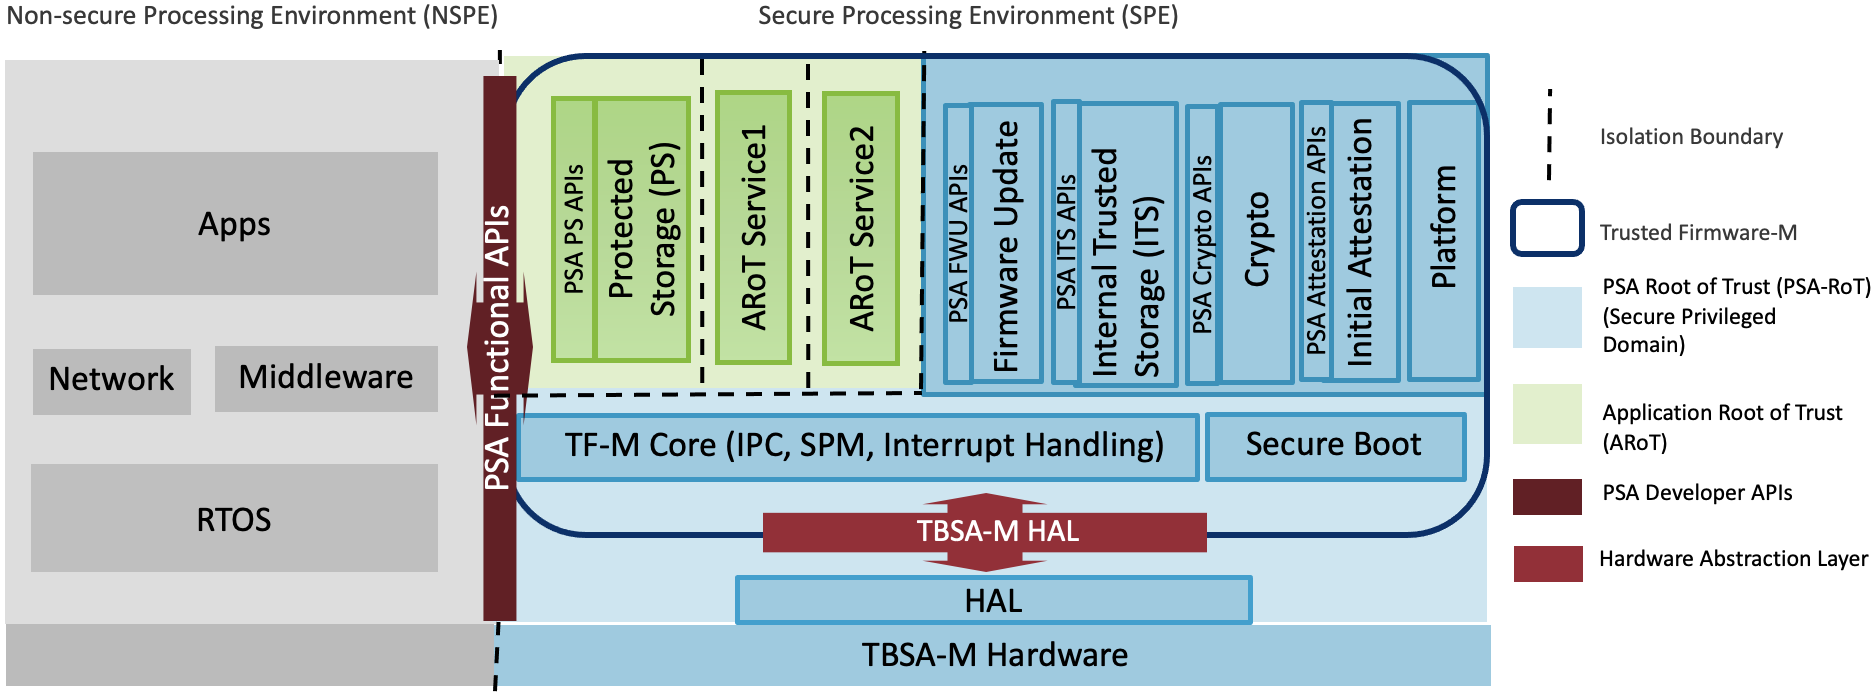
\includegraphics[scale=0.24]{graph/readme_tfm_v8.png}
    \caption{Trusted Firmware-M架构图}
\end{figure}
\par 在Trusted Firmware-M的背景下,安全启动负责在固件映像被加载和执行之前验证其真实性和完整性。它通过根据设备安全引导固件中存储的一组受信任的密钥检查固件映像的数字签名来执行此验证。安全启动可以对SPE (Secure Processing Environment)和 NSPE (Non-Secure Processing Environment)固件映像进行身份验证。NSPE映像在设备的非安全世界中执行,而SPE映像在安全世界中执行。如果固件映像未通过Secure Boot验证,则会被拒绝,设备将无法执行它。这可以防止攻击者在设备上执行未经授权的代码,从而保护设备及其数据免受恶意活动的侵害。
\par TF-M内核是TF-M的主要组成部分之一,它是一个基于微内核的安全操作系统内核。TF-M core的主要功能是提供安全隔离、通信控制和安全执行,主要模块包括IPC、SPM、Interrupt Handling。其中,IPC 用于在SPE和 NSPE之间进行通信。它提供了一种安全的方式,以便在受保护的环境内传递数据和控制信息。SPM用于管理和控制在SPE中运行的各个安全分区。SPM使得多个安全分区可以在同一硬件平台上运行,并且可以互相隔离。Interrupt Handling用于管理和处理来自设备的中断请求。TF-M内核通过在SPE和NSPE之间传递中断请求,确保了所有中断的安全处理。TF-M内核还包括一些其他的辅助模块,比如Secure Entry/Exit和Secure Attribution等,用于在SPE和NSPE之间进行安全的上下文切换和资源分配。
\par 安全服务负责向安全/非安全世界提供具有较高安全需求的功能实现并由安全内核负责对其进行调用,如安全储存、安全启动、加密等。每一个安全服务具有唯一标识符SID(Service ID)且有统一的函数调用入口。为统一调用接口,每个安全服务都可以通过SID和version两个参数被非安全世界用户进行调用,其中,SID参数是要调用的安全服务的唯一标识符,version是请求的信任根服务版本。NSPE的用户通过PSA API发送请求后,由SPM将请求打包成消息并转发到相应服务处理程序的函数。
\par TF-M拥有特定的隔离机制,以保护一个保护域的信息免受从其他域访问,故TF-M中不同区域间的访问需要特定的PSA API来实现,后续将详细解释TF-M的通信机制。

\paragraph{TF-M隔离机制}PSA针对不同设备的安全性、性能、成本提出了三个级别的隔离,如下图所示。第一级隔离将SPE与NSPE隔离开,NSPE不能访问SPE的资源,需要由PSA client API访问特定的服务。第二级隔离在第一级隔离的基础上,引入了PSA RoT和Application RoT隔离边界。这两类服务不能访问各自的资源,需要由PSA API访问对方的服务。第三级隔离在前两级的基础上引入了对每个安全分区之间的隔离边界,实现对所有安全分区的隔离,其是最高级别的隔离。
\begin{figure}
    \centering
    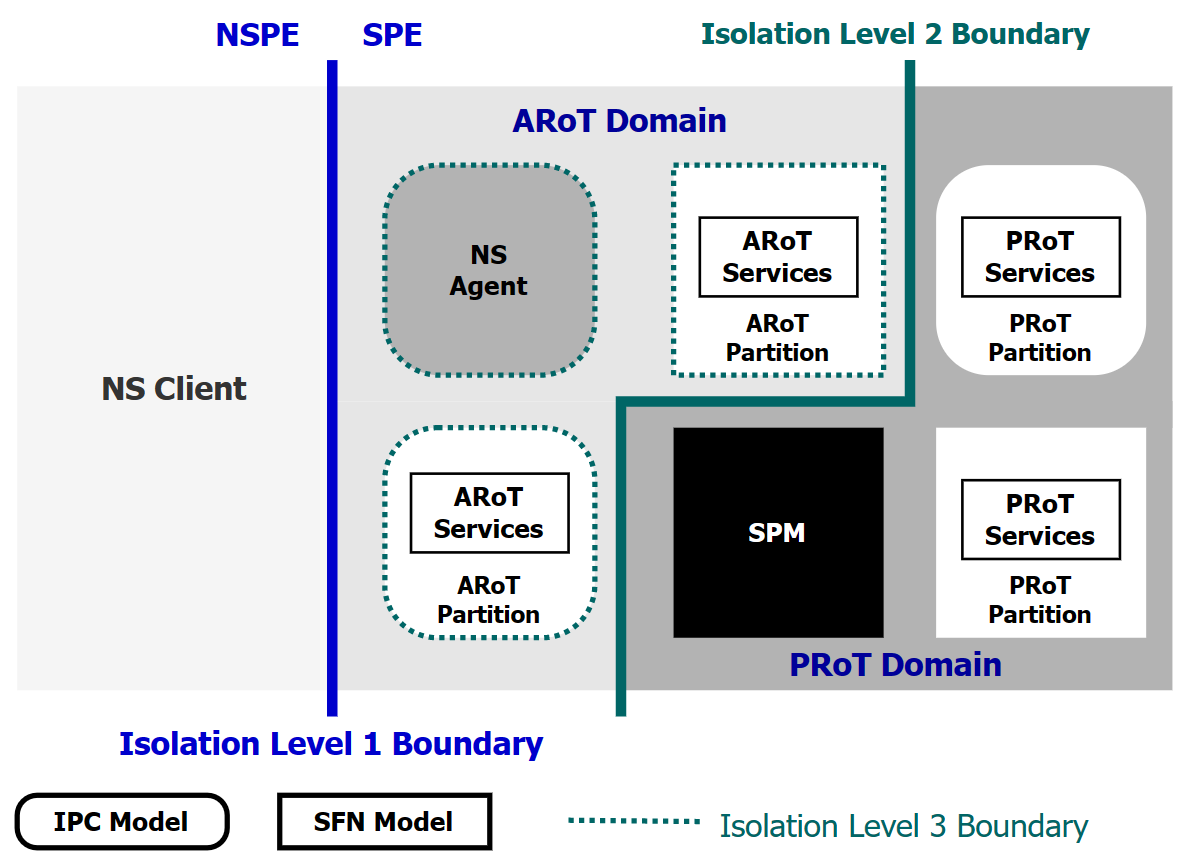
\includegraphics[scale=0.24]{graph/isolation.png}
    \caption{TF-M隔离机制}
\end{figure}

\subsection{实验成果展示}
\section{作品测试与分析}
\subsection{测试方案}
\subsection{测试环境搭建}
\subsection{测试数据及分析}
\section{创新性说明}
\section{总结}
\bibliographystyle{plain}
\bibliography{ref}
\end{document}